\documentclass[a4paper]{article}

%% Language and font encodings
\usepackage[english]{babel}
\usepackage[utf8x]{inputenc}
\usepackage[T1]{fontenc}
\setlength{\parindent}{0em}
\setlength{\parskip}{1em}
\usepackage{framed,lipsum}
\usepackage[dvipsnames]{xcolor}
\usepackage{minted}

%% Sets page size and margins
% \usepackage[a4paper,top=3cm,bottom=2cm,left=3cm,right=3cm,marginparwidth=1.75cm]{geometry}
\usepackage[a4paper,top=2cm,bottom=2cm,left=1.5cm,right=1.5cm,marginparwidth=1.5cm]{geometry}



%% Useful packages
\usepackage{hyperref}
\hypersetup{
	colorlinks=true,
	linkcolor=blue,
	filecolor=magenta,      
	urlcolor=blue,
}
%\usepackage{amsmath}
\usepackage{graphicx}
%\usepackage[colorinlistoftodos]{todonotes}
%\usepackage[colorlinks=true, allcolors=blue]{hyperref}

\title{\textbf{Machine Learning Engineering Nanodegree} \\
\Large Capstone Project Proposal}
\author{Zhiwei Lin}
\date{\today}

\begin{document}
	\maketitle
	
	\section*{Domain Background}
	
	This project is to investigate a docked bike-sharing system in San Francisco Bay Area, data collected during 2013-2015 when this system just got launched. Different from bike rentals serving for casual riding over several hours or days, bike sharing focuses more on providing bike service on short trips to solve the "last mile" problem, especially for metropolitan areas. The bike sharing service brings convenience to people in situations where neither driving or walking is efficient.
	
	While dock-less bike sharing systems are expanding over the world with dominant number of share-bikes, dock-based bike sharing systems are still the "mainstream" in the US. Even San Francisco Bay Area, currently the technology innovation center of the world, \href{https://www.recode.net/2017/10/23/16496908/bike-sharing-dockless-limebike-ofo-motivate-citi-bike-spin}{only recently starts seeing the wave of the dock-less bike sharing systems}. It is not foreseeable in the near future whether the dock-based system will be fiercely challenged in the US by the dock-less system due to the nature of less populous cities and the existing somewhat mature business model for the docked system. On the other hand, investigation into the dock-based system is a good attempt if one would like to explore further how to improve a dock-less system. To some extent, the dock-less system can be viewed an extension of a dock-based system with a much larger number of stations.
	
	Bike sharing is becoming more and more popular around the world. To improve the bike-sharing systems to make people's life easier and more enjoyable, it is worth studying this system closely, especially on how people use the share-bikes. There are several datasets available on Kaggle on bike sharing with many kinds of analyses. I will focus on the dataset for \href{https://www.kaggle.com/benhamner/sf-bay-area-bike-share}{SF Bay Area Bike Share} as the data are informative and relatively new.
	
	There is also some helpful discussion in academia reviewed by this paper published last year on the bike sharing:
	\href{https://nacto.org/wp-content/uploads/2016/02/2016_Fishman_Bikeshare-A-Review-of-Recent-Literature.pdf}{Bikeshare: A Review of Recent Literature}.
	
		
	\section*{Problem Statement}
	
	The dataset contains files with structured data, in csv and sqlite formats. Some data are in time series, but they will not be treated as time-series data for training. The assumption is that macroscopically people's behavior on share-bike usage of a specific time section does not depend on the previous one if the sections are carefully defined. Two major problems will be addressed:
	
	\begin{itemize}
		\item How do people use share-bikes at different time periods? Specifically, trip patterns on weekdays, weekends and holidays will be investigated. During one day, how many sections are there with unique characteristics? For instance, one may naturally think of morning, afternoon, evening, late night as four distinct periods for human activities, including the bike riding.
		
		The original data will be transformed with the divisions within a day obtained from the data exploration. The knowledge learned from the training set will be applied to predict the number of trips on test set. The outputs are continuous values, so this is a regression problem. 
		
		It is very important to predict the demand of share-bikes at several key sections during a day on each specific date. In particular, high peaks of the share-bike usage need to be handled well in order to ensure an efficient system. The strategy to re-balancing docks on all the stations is somewhat critical for the bike-sharing company to operate their business.
		
		\item What are the different behaviors between long-term users ("Subscriber") and short-term users ("Customer")? Can we predict whether the biker is a Subscriber or a Customer based on certain features of a specific trip?
		
		Relevant features from the original data will be selected to form an appropriate dataset and then the corresponding training and test sets. A trained model will be used to predict a subscriber or a short-term user on the test set. The accuracy of prediction will be used as the main metric. The outputs are two possible class labels, so this is a classification problem. 
		
		For this problem, the goal is actually not on the result of prediction accuracy, but rather on how to interpret the predicted results when the accuracy is high enough to show strong correlation between the label and the features. Most important features will be extracted to form guidelines to assist bike-sharing companies to come up with proper promotions to convert short-term customers to long-term subscribers.
		
	\end{itemize}
	
	\section*{Datasets and Inputs}
	
	The original data used come from \href{https://www.kaggle.com/benhamner/sf-bay-area-bike-share}{SF Bay Area Bike Share} from Kaggle. The dataset can be downloaded from \href{(https://www.kaggle.com/benhamner/sf-bay-area-bike-share/downloads/sf-bay-area-bike-share.zip)}{this link}. This dataset is directly related to the problems that are targeted. It includes all "anonymized bike trip data from August 2013 to August 2015" of the San Francisco Bay Area Bike Share program.
		
	The size of original data is 660MB when downloaded and about 5GB when unzipped.  After the data preprocessing to distill the useful information, the data size is shrunk to less than 150MB, which is the one that will be used to create the two datasets for the two respective problems mentioned above. The dataset contains information for bike stations [shape: (70, 7)], status of stations [shape: (2109513, 4)], trips [shape: (669959, 11)] and weather [shape: (3665, 24)]. These are all useful in data exploration.
	
	There are time series included in the preprocessed data. The status, trip and weather all have timestamps on each event. However, this is not necessary a time-series machine learning problem. The timestamps will be converted to categorical columns, e.g. a column showing whether a day is a working day or not and a column showing characteristic time sections during one day. After some data cleaning and manipulation on four individual data, the processed data will be combined to form a complete dataset. Two variations of this dataset will be further created for the two problems: 1. data within the same time section will be aggregated and a label column of trip counts will be created for the regression problem; 2. a label column of the subscriber type will be selected for the classification problem.
	
	The test set will be created based on the assumption that share-bike usage pattern of a specific time section does not depend on the previous one. Inevitably there will still be some dependence among sections during one day, but each day can be treated as totally independent because of the natural cycle of human activities (people need to sleep). Therefore, the dataset will be randomly divided into training and test sets with the splitting unit being one day. 
	
	\section*{Solution Statement}
	
	For the trip count prediction problem, the data will first be explored to show trip counts with respect to several variables, e.g. weather condition, time during a day, weekday or weekend, location of the station, available bikes, etc. The data will then be combined and transformed to form a new dataset with the count of trips as the labeled column. A regression method, most likely a linear model, will be built. The root mean squared logarithmic error will be calculated to test the generality of the model.
	
	The subscriber prediction problem is a binary classification problem, so the labeled column will contain only true and false values. Different classification models will be explored, with a focus on interpretable algorithms like logistic regression, Naive Bayes, decision tree as understanding the underlying reasons is the goal of this analysis. The prediction accuracy on the test set will be calculated to test the model's performance. Then the results will be discussed to extract the most relevant features for decision making to bike sharing companies.
	
	For both problems, cross validations will be done on the training set to obtain a better model. The splittings of the training set will have one day as the unit according to the previous discussion on the test set generation. As suggested by the first reviewer, a special splitting method (sklearn's \href{http://scikit-learn.org/stable/modules/generated/sklearn.model_selection.TimeSeriesSplit.html}{TimeSeriesSplit}), with the validation set always later in time than the training set, will also be investigated to check whether there is a significant data leakage.
		
	\section*{Benchmark Model}
	
	There are some discussions around this data on Kaggle. The closest analysis to my first set problem is from a notebook named \href{https://www.kaggle.com/currie32/a-model-to-predict-number-of-daily-trips/notebook}{A Model to Predict Number of Daily Trips}. A weighted model from random forest regression, gradient boosting regression and XGBoost is used for the prediction, which can be considered a benchmark model to compare with. The author concludes that:
	
	\begin{leftbar}
		\texttt{My model has a median absolute error of almost 47 trips per day. This should give the company operating this service a good, general estimate of the traffic that will occur each day.}
	\end{leftbar}
	
	Another benchmark result comes from a different bike-sharing dataset: \href{https://www.kaggle.com/c/bike-sharing-demand/}{Bike Sharing Demand}. Also using the Root Mean Squared Logarithmic Error as the metric, the best score on its \href{https://www.kaggle.com/c/bike-sharing-demand/leaderboard}{public leaderboard} is 0.33756. The model is not open to public though.
	
	Note that slightly different problems are targeted by the above-mentioned two solutions. So the result cannot be directly compared. Thus, a model that randomly selects a trip count from historical data of the same time section in a day will be established as another benchmark model as a "sanity" check baseline.
	
	As for the second problem I set, no discussion exists to my best knowledge. A plain random guess can serve as the benchmark model.
	
	\section*{Evaluation Metrics}
	
	For the regression problem (predicting the number of bikes in demand), the Root Mean Squared Logarithmic Error (RMSLE) will be used as the evaluation metrics as suggested by Kaggle for the project \href{(https://www.kaggle.com/c/bike-sharing-demand#evaluation)}{Bike Sharing Demand}. The RMSLE is calculated as 
	\begin{equation}
	RMSLE = \sqrt{\frac{1}{n}\sum_{i=1}^{n}(\log(p_i + 1) - \log(a_i + 1))^2}
	\end{equation}
	
	Where:
	\begin{itemize}
		\item $n$ is the number of entries in the test set
		\item $p_i$ is the predicted count
		\item $a_i$ is the actual count
		\item $\log(x)$ is the natural logarithm
	\end{itemize}
		
	For the classification problem (predicting the user as a subscriber or not), the accuracy of the predictions will be used as the metric. The accuracy is calculated as the ratio of the number of correctly predicted data points to the total number of data points in the test set:
	\begin{equation}
	Accuracy = \frac{\sum_{i=1}^{N} (m_i == n_i)}{N}
	\end{equation}
	
	Where:
	\begin{itemize}
		\item $m_i$ is the predicted category of $i^{th}$ row in the test set
		\item $n_i$ is the labeled category of $i^{th}$ row in the test set
		\item $N$ is the number of entries in the test set
	\end{itemize}
	
	\section*{Project Design}
	
	First of all, the original data require some "compression" in order for Pandas Dataframe to handle. The status.csv data cannot be loaded by Pandas's read\_csv function, even if the file size is only 2GB when I have 8GB computer memory. The original status data record the number of bikes and docks available for given station; each entry is recorded for every minute. The frequent data recording is not necessary for data analysis, because the status of each station does not necessarily change per minute. Redundant records for which status remains the same can be removed without sacrificing the data integrity. 
	
	Fortunately, an SQL database is also provided. It contains identical information with those csv files. Using SQL commands, data can be loaded piece by piece (by stations) to Pandas Dataframe for data compression. After this operation, a file "status\_change.csv" is created with the size less than 60MB. Compared to the "status.csv" file of 2GB, a compression ratio of more than 30 is observed by preprocessing the data. Pandas can easily handle this data file. See below the excerpted Python code for data compression:
	
	\begin{minted}
	[
	tabsize=4,
	frame=lines,
	framesep=2mm,
	baselinestretch=1.2,
	fontsize=\footnotesize,
	stripall=true,
	linenos
	]
	{python}
	
def bike_status(station_id, sql_conn):
	status = pd.read_sql_query(f"SELECT * FROM status WHERE station_id = {station_id} ORDER BY time", con=sql_conn)
	status_shift = status.shift(-1)
	status_compact = status[(status.bikes_available != status_shift.bikes_available) 
	|(status.docks_available != status_shift.docks_available)]
	return status_compact
	
status_list = [bike_status(station_id, conn) for station_id in tqdm(station.id)]
status = pd.concat(status_list, ignore_index=True)
status.to_csv("status_change.csv", index=False)
	
\end{minted}
	
	Another important thing to check before applying any algorithm to the data is whether all these stations are located closely to each other. If two stations are too far apart, it becomes unlikely that a user will ride the bike from one station to the other. Bike stations are marked on Google Map as shown in Figure \ref{fig:map}:
	
	\begin{figure}
		\centering
		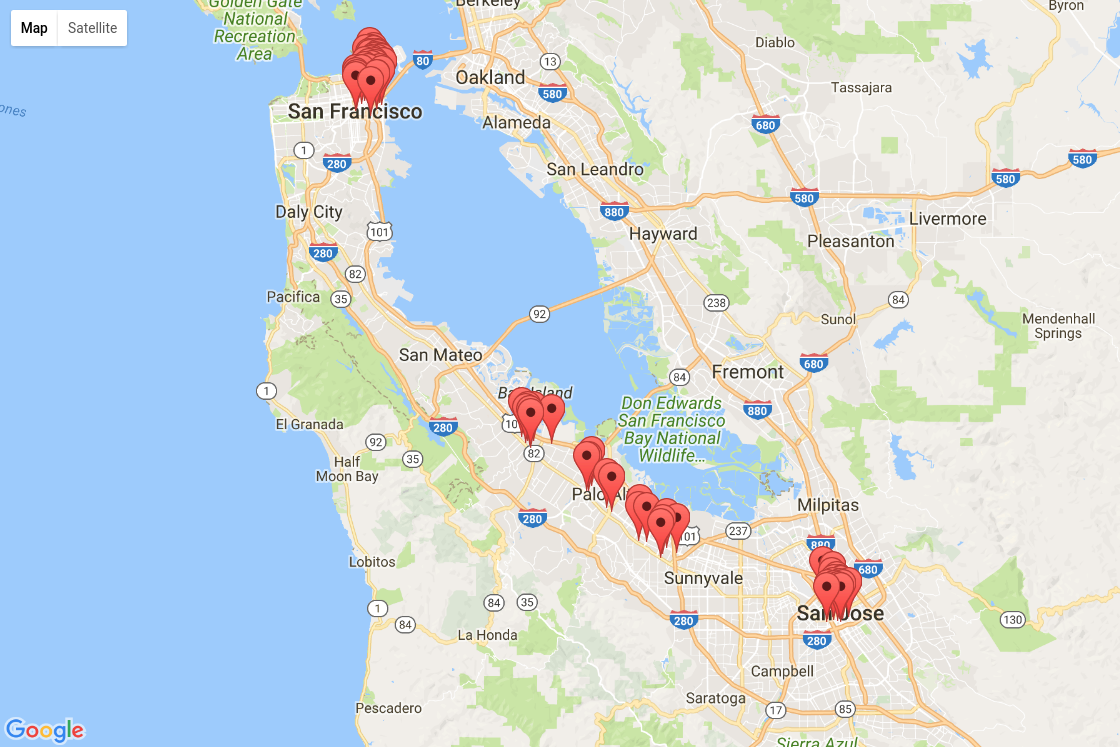
\includegraphics[width=0.8\textwidth]{Station_Map.png}
		\caption{\label{fig:map}The station map is generated from the station.csv data via JavaScript.}
	\end{figure}
	
	From the station map, it is clear that the stations can be loosely divided into five sections, with two major centers in San Francisco and San Jose. Clustering model will be applied to the coordinates for stations to group them into separate subsets. Moreover, statistics will be done on trips between different stations to see if the clustering makes sense. These subsets may have different patterns, which will be investigated further in data exploration.
	
	Some other aspects of the data are worth looking into. For example, the weather data have too many columns, which may lead to the curse of dimensionality. Many weather variables can be highly correlated to each other. Only one of the features with strong correlation should be kept. Ideally the final dataset will have orthogonal data columns. Another example is the zip codes. Zip code formatting is not consistently five-digit. Zip codes with less than five digits need to add zeros to the front, while those with more than five digits need to be truncated. In addition, peaks of bike usage will be plotted to define characteristic periods during a day. Null data points requires filling with reasonable values or just deleting. Data outliers need to be carefully dealt with. Categorical features will be properly encoded (e.g. one-hot). Normalization may be necessary for certain features. So on and so forth.
	
	Then, data will be combined to form a complete dataset based on relational features among them, such as the station id, the date and time of the trip, location, etc. This dataset will be further transformed to two variations to accommodate the investigation of the two problems:
	
	\begin{enumerate}
		\item The regression problem to predict the bike demand. Data will be aggregated according to the period of time defined earlier. A column of trip count during each period will be added: this will be the label column. 
		\item The classification problem to predict the subscription. The "subscription\_type" column will be used as the label column. The values will be replaced as 1 (True) or 0 (False).
	\end{enumerate}
		
	After all the data cleaning and manipulation, the respective dataset for the two problems will be divided into a training set and a test set on a daily basis. The metrics will be defined. Proper supervised machine learning algorithms for regression and classification will be applied. K-fold cross validation will be done properly to improve the model. The final model will be applied to the test set; the performance of the model will be judged by the defined metrics. The results will be discussed and interpretation of the model will be provided if possible. Lastly, conclusions will be drawn to assist the decision making for bike sharing companies.

\end{document}